\documentclass[12pt]{standalone}
\usepackage{tikz}

\begin{document}
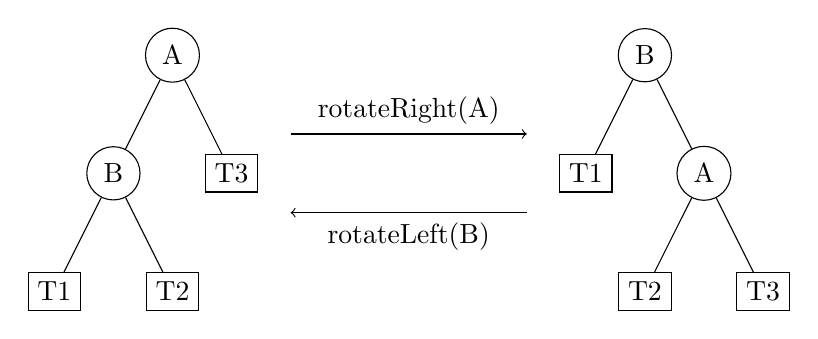
\begin{tikzpicture}

    \tikzstyle{nodebase}=[align=center, text centered, draw]
    \tikzstyle{node_a}=[nodebase, circle]
    \tikzstyle{subtree}=[nodebase, rectangle]

    \node [node_a] at (-3,0) {A}
    child {node [node_a] {B}
            child {node [subtree] {T1}}
            child {node [subtree] {T2}}}
    child {node [subtree] {T3}};

    \node [node_a] at (3,0) {B}
    child {node [subtree] {T1}}
    child {node [node_a] {A}
            child {node [subtree] {T2}}
            child {node [subtree] {T3}}};

    \draw[->] (-1.5,-1) -- ++(3,0) node[midway, above] {rotateRight(A)};
    \draw[->] (1.5,-2) -- ++(-3,0) node[midway, below] {rotateLeft(B)};

\end{tikzpicture}
\end{document}
